%%%%%%%%%%%%%%%%%%%%%%%%%%%%%%%%%%%%%%%%%
% Beamer Presentation
% LaTeX Template
% Version 2.0 (March 8, 2022)
%
% This template originates from:
% https://www.LaTeXTemplates.com
%
% Author:
% Vel (vel@latextemplates.com)
%
% License:
% CC BY-NC-SA 4.0 (https://creativecommons.org/licenses/by-nc-sa/4.0/)
%
%%%%%%%%%%%%%%%%%%%%%%%%%%%%%%%%%%%%%%%%%

%%%%%%%%%%%%%%%%%%%%%%%%%%%%%%%%%%%%%%%%%
% This presentation template is an adaptation of the template mentioned above. It has been created by Giovanni Spadaro and it is available on GitHub (https://github.com/Giovo17/presentation-template-unict-lm-data).
%%%%%%%%%%%%%%%%%%%%%%%%%%%%%%%%%%%%%%%%%

%----------------------------------------------------------------------------------------
%	PACKAGES AND OTHER DOCUMENT CONFIGURATIONS
%----------------------------------------------------------------------------------------

\documentclass[
	11pt, % Set the default font size, options include: 8pt, 9pt, 10pt, 11pt, 12pt, 14pt, 17pt, 20pt
	%t, % Uncomment to vertically align all slide content to the top of the slide, rather than the default centered
	%aspectratio=169, % Uncomment to set the aspect ratio to a 16:9 ratio which matches the aspect ratio of 1080p and 4K screens and projectors
]{beamer}

\graphicspath{{img/}} % Specifies where to look for included images (trailing slash required)

\usepackage{booktabs} % Allows the use of \toprule, \midrule and \bottomrule for better rules in tables

%----------------------------------------------------------------------------------------
%	SELECT LAYOUT THEME
%----------------------------------------------------------------------------------------

% Beamer comes with a number of default layout themes which change the colors and layouts of slides. Below is a list of all themes available, uncomment each in turn to see what they look like.

%\usetheme{default}
%\usetheme{AnnArbor}
%\usetheme{Antibes}
%\usetheme{Bergen}
%\usetheme{Berkeley}
%\usetheme{Berlin}
\usetheme{Boadilla}
%\usepackage{enumitem}
\usepackage{array}
%\usetheme{CambridgeUS}
%\usetheme{Copenhagen}
%\usetheme{Darmstadt}
%\usetheme{Dresden}
%\usetheme{Frankfurt}
%\usetheme{Goettingen}
%\usetheme{Hannover}
%\usetheme{Ilmenau}
%\usetheme{JuanLesPins}
%\usetheme{Luebeck}
%\usetheme{Madrid}
%\usetheme{Malmoe}
%\usetheme{Marburg}
%\usetheme{Montpellier}
%\usetheme{PaloAlto}
%\usetheme{Pittsburgh}
%\usetheme{Rochester}
%\usetheme{Singapore}
%\usetheme{Szeged}
%\usetheme{Warsaw}

%----------------------------------------------------------------------------------------
%	SELECT COLOR THEME
%----------------------------------------------------------------------------------------

% Beamer comes with a number of color themes that can be applied to any layout theme to change its colors. Uncomment each of these in turn to see how they change the colors of your selected layout theme.

%\usecolortheme{albatross}
%\usecolortheme{beaver}   % red
%\usecolortheme{beetle}
%\usecolortheme{crane}   % yellow
%\usecolortheme{dolphin}  % purple
%\usecolortheme{dove}   % white
%\usecolortheme{fly}   % grey
%\usecolortheme{lily}   % purple
%\usecolortheme{monarca}   % yellow background and black
%\usecolortheme{seagull}
%\usecolortheme{seahorse}
%\usecolortheme{spruce}   % green
\usecolortheme{whale}
%\usecolortheme{wolverine}

%----------------------------------------------------------------------------------------
%	SELECT FONT THEME & FONTS
%----------------------------------------------------------------------------------------

% Beamer comes with several font themes to easily change the fonts used in various parts of the presentation. Review the comments beside each one to decide if you would like to use it. Note that additional options can be specified for several of these font themes, consult the beamer documentation for more information.

\usefonttheme{default} % Typeset using the default sans serif font
%\usefonttheme{serif} % Typeset using the default serif font (make sure a sans font isn't being set as the default font if you use this option!)
%\usefonttheme{structurebold} % Typeset important structure text (titles, headlines, footlines, sidebar, etc) in bold
%\usefonttheme{structureitalicserif} % Typeset important structure text (titles, headlines, footlines, sidebar, etc) in italic serif
%\usefonttheme{structuresmallcapsserif} % Typeset important structure text (titles, headlines, footlines, sidebar, etc) in small caps serif

%------------------------------------------------

%\usepackage{mathptmx} % Use the Times font for serif text
\usepackage{palatino} % Use the Palatino font for serif text

%\usepackage{helvet} % Use the Helvetica font for sans serif text
\usepackage[default]{opensans} % Use the Open Sans font for sans serif text
%\usepackage[default]{FiraSans} % Use the Fira Sans font for sans serif text
%\usepackage[default]{lato} % Use the Lato font for sans serif text

%----------------------------------------------------------------------------------------
%	SELECT INNER THEME
%----------------------------------------------------------------------------------------

% Inner themes change the styling of internal slide elements, for example: bullet points, blocks, bibliography entries, title pages, theorems, etc. Uncomment each theme in turn to see what changes it makes to your presentation.

%\useinnertheme{default}
\useinnertheme{circles}
%\useinnertheme{rectangles}
%\useinnertheme{rounded}
%\useinnertheme{inmargin}

%----------------------------------------------------------------------------------------
%	SELECT OUTER THEME
%----------------------------------------------------------------------------------------

% Outer themes change the overall layout of slides, such as: header and footer lines, sidebars and slide titles. Uncomment each theme in turn to see what changes it makes to your presentation.

%\useoutertheme{default}
%\useoutertheme{infolines}
\useoutertheme{miniframes}
%\useoutertheme{smoothbars}
%\useoutertheme{sidebar}
%\useoutertheme{split}
%\useoutertheme{shadow}
%\useoutertheme{tree}
%\useoutertheme{smoothtree}

\definecolor{darkBlue}{rgb}{0,0,0.31}
%\definecolor{darkBlue}{rgb}{0,0,0.5}
\definecolor{munsell}{rgb}{0.0, 0.5, 0.69}
\definecolor{indigo}{rgb}{0.0, 0.25, 0.42}
\definecolor{codeblue}{rgb}{0.25,0.5,0.5}
\definecolor{backcolour}{rgb}{0.95,0.95,0.92}
\definecolor{commentblue}{rgb}{0.3,0.3,0.6}
\definecolor{keywordblue}{rgb}{0.2,0.2,0.7}
\definecolor{stringblue}{rgb}{0.15,0.2,0.9}

%\setbeamertemplate{footline} % Uncomment this line to remove the footer line in all slides
%\setbeamertemplate{footline}[page number] % Uncomment this line to replace the footer line in all slides with a simple slide count

%\setbeamertemplate{navigation symbols}{} % Uncomment this line to remove the navigation symbols from the bottom of all slides

% Establecer Latin Modern Sans Serif como la fuente predeterminada
\renewcommand*\familydefault{\sfdefault} % Cambia la fuente predeterminada a sans-serif
\usepackage[T1]{fontenc} % Codificación de la fuente
\usepackage{lmodern} % Carga la fuente Latin Modern\textbf{}
\usepackage{tikz}
\usetikzlibrary{positioning, arrows.meta}
\usepackage{svg}
\usepackage{listings}
\lstdefinestyle{bluepythonstyle}{
	language=Python,
	basicstyle=\ttfamily\small,
	commentstyle=\color{commentblue},
	keywordstyle=\color{keywordblue},
	numberstyle=\tiny\color{codeblue},
	stringstyle=\color{stringblue},
	backgroundcolor=\color{backcolour},
	breaklines=true,
	captionpos=b,
	abovecaptionskip=1\baselineskip,
	showstringspaces=false,
	frame=lines,
	numbers=left,
	xleftmargin=\parindent,
	tabsize=4
}
\lstset{style=bluepythonstyle}

%----------------------------------------------------------------------------------------
%	PRESENTATION INFORMATION
%----------------------------------------------------------------------------------------

\title[Caminante Aleatorio]{\textbf{Caminante Aleatorio}} % The short title in the optional parameter appears at the bottom of every slide, the full title in the main parameter is only on the title page

%\subtitle{Optional Subtitle} % Presentation subtitle, remove this command if a subtitle isn't required

\institute[]{\textit{Instituto Politécnico Nacional \\ Centro de Investigación en Computación}}

\author[Rodrigo Trejo]{Rodrigo Trejo} % Presenter name(s), the optional parameter can contain a shortened version to appear on the bottom of every slide, while the main parameter will appear on the title slide


 % Your institution, the optional parameter can be used for the institution shorthand and will appear on the bottom of every slide after author names, while the required parameter is used on the title slide and can include your email address or additional information on separate lines

 % Presentation date or conference/meeting name, the optional parameter can contain a shortened version to appear on the bottom of every slide, while the required parameter value is output to the title slide

\usepackage{pgfplots}
\pgfplotsset{compat=newest}
%----------------------------------------------------------------------------------------

\begin{document}

%----------------------------------------------------------------------------------------
%	TITLE SLIDE
%----------------------------------------------------------------------------------------

\begin{frame}


	\titlepage % Output the title slide, automatically created using the text entered in the PRESENTATION INFORMATION block above
\end{frame}

%----------------------------------------------------------------------------------------
%	TABLE OF CONTENTS SLIDE
%----------------------------------------------------------------------------------------

% The table of contents outputs the sections and subsections that appear in your presentation, specified with the standard \section and \subsection commands. You may either display all sections and subsections on one slide with \tableofcontents, or display each section at a time on subsequent slides with \tableofcontents[pausesections]. The latter is useful if you want to step through each section and mention what you will discuss.

\begin{frame}
	\frametitle{Presentation Overview} % Slide title, remove this command for no title
	
	\tableofcontents % Output the table of contents (all sections on one slide)
	%\tableofcontents[pausesections] % Output the table of contents (break sections up across separate slides)
\end{frame}

%----------------------------------------------------------------------------------------
%	PRESENTATION BODY SLIDES
%----------------------------------------------------------------------------------------



\section{Generación de números aleatorios} % Sections are added in order to organize your presentation into discrete blocks, all sections and subsections are automatically output to the table of contents as an overview of the talk but NOT output in the presentation as separate slides

%------------------------------------------------

\begin{frame}
	\frametitle{Distribución Uniforme}
	
	    \begin{columns}
		
		% Columna de la izquierda
		\begin{column}{0.5\textwidth} % Ajusta la proporción según necesites
			\begin{figure}
				\centering
				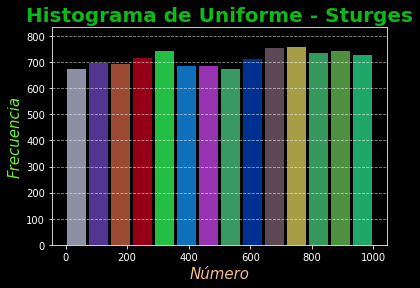
\includegraphics[width=\textwidth]{hist_uniform_Sturges} % Asegúrate de cambiar la ruta a la ubicación de tu imagen
				\caption{Histograma de distribución uniforme.}
			\end{figure}
		\end{column}
		
		% Columna de la derecha
		\begin{column}{0.5\textwidth} % Ajusta la proporción según necesites
			\begin{itemize}
				\item Se generó un archivo de \textit{10000} números aleatorios uniformemente distribuidos. 
				\item Se almacenan como \texttt{randomsUnifome.txt}
			\end{itemize}
		\end{column}
	\end{columns}
\end{frame}

%------------------------------------------------



\section{Transformaciones}

\begin{frame}
	\frametitle{Transformación a distribución normal}
		
		\begin{columns}
			
			% Columna de la izquierda
			\begin{column}{0.5\textwidth} % Ajusta la proporción según necesites
				\begin{figure}
					\centering
					\includegraphics[width=\textwidth]{hist_normal_rice} % Asegúrate de cambiar la ruta a la ubicación de tu imagen
					\caption{Histograma de distribución normal.}
				\end{figure}
			\end{column}
			
			% Columna de la derecha
			\begin{column}{0.5\textwidth} % Ajusta la proporción según necesites
				\begin{itemize}
					\item La transformación de una distribución uniforme a normal se realiza mediante la función de error inversa.
					\item Convierte cuantiles uniformes en valores de una distribución normal, ajustándolos después según la media y desviación estándar deseadas.
					\item Facilita la interpretación estadística, mapeando probabilidades uniformes a la escala de la normalidad.
				\end{itemize}
			\end{column}
		\end{columns}
\end{frame}


\begin{frame}
	\frametitle{Transformación a distribución gamma}
	
	\begin{columns}
		% Columna de la derecha
		\begin{column}{0.5\textwidth} % Ajusta la proporción según necesites
			\begin{itemize}
				\item El método de aceptación-rechazo genera variables aleatorias Gamma a partir de distribuciones uniformes. 
				\item Se calcula un valor \(y\) a partir de una variable uniforme y se compara con una función de densidad proporcional a la distribución Gamma. Si \(y\) es aceptado según un criterio de comparación, se escala y se retorna como resultado.
			\end{itemize}
			
		\end{column}

	
	
	% Columna de la izquierda
	\begin{column}{0.5\textwidth} % Ajusta la proporción según necesites
		\begin{figure}
			\centering
			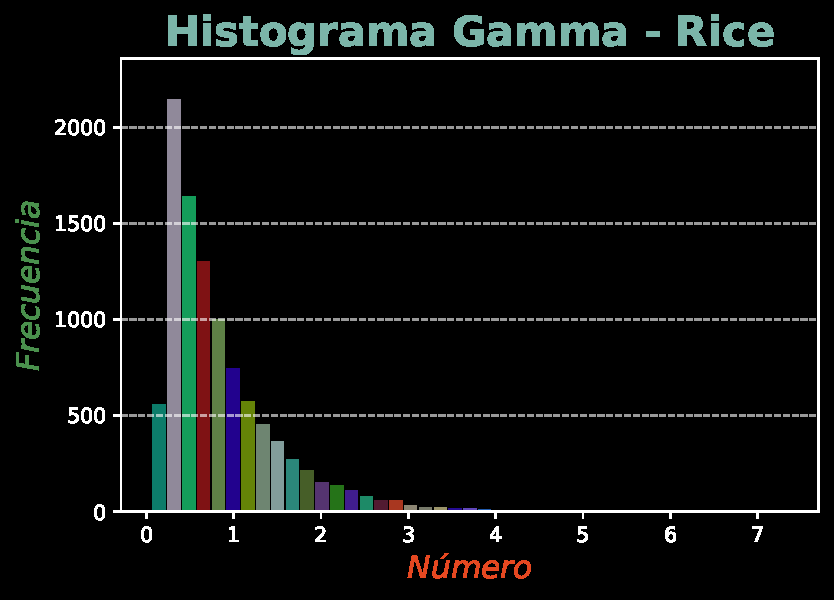
\includegraphics[width=\textwidth]{hist_gamma_Rice} % Asegúrate de cambiar la ruta a la ubicación de tu imagen
			\caption{Histograma de distribución gamma.}
		\end{figure}
	\end{column}
	\end{columns}
\end{frame}


\begin{frame}
	\frametitle{Transformación lineal}
	
	\begin{columns}
		
		% Columna de la izquierda
		\begin{column}{0.5\textwidth} % Ajusta la proporción según necesites
			\begin{figure}
				\centering
				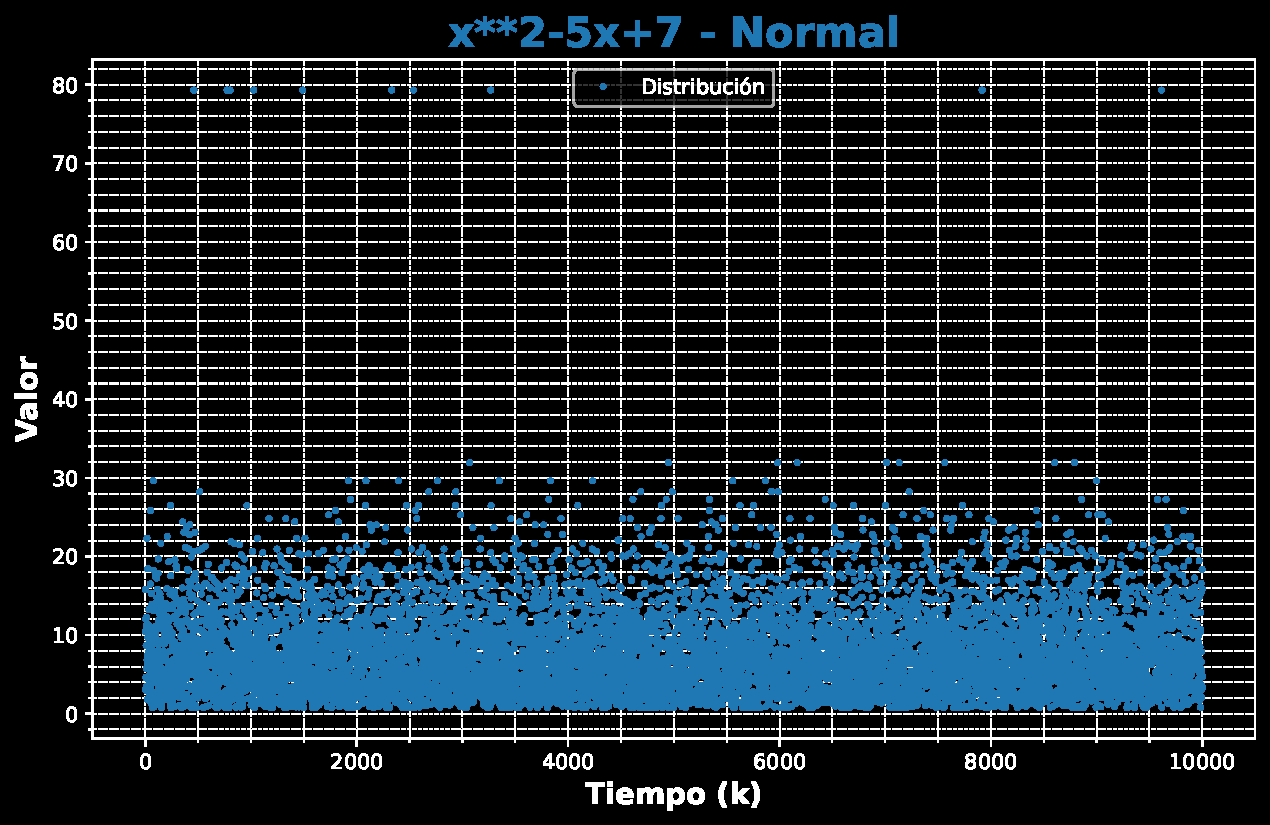
\includegraphics[width=\textwidth]{cuad_normal1} % Asegúrate de cambiar la ruta a la ubicación de tu imagen
				\caption{Gráfica de la serie de tiempo para el polinomio $x^2-5x+7$.}
			\end{figure}
		\end{column}
		
		% Columna de la derecha
		\begin{column}{0.5\textwidth} % Ajusta la proporción según necesites
			\begin{figure}
				\centering
				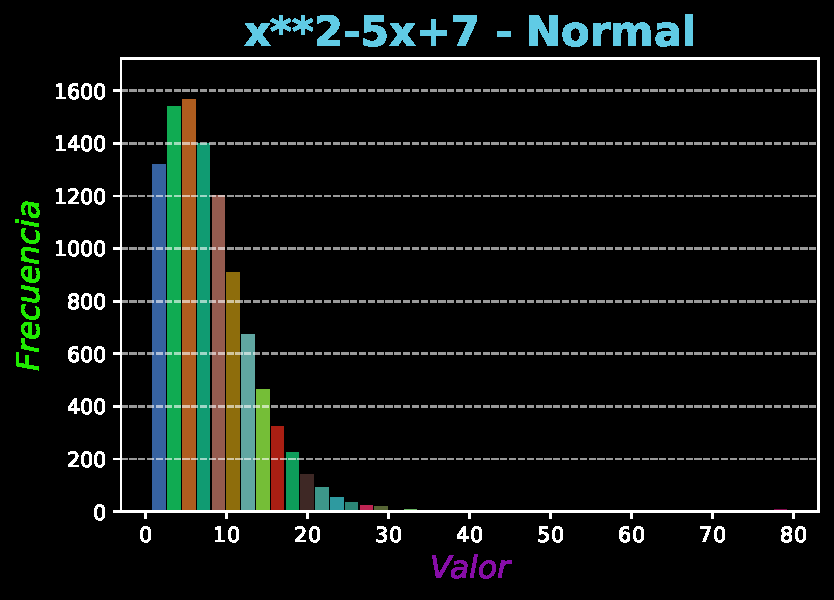
\includegraphics[width=\textwidth]{cuad_normal2} % Asegúrate de cambiar la ruta a la ubicación de tu imagen
				\caption{Distribución de los datos.}
			\end{figure}
		\end{column}
	\end{columns}
\end{frame}


\begin{frame}
	\frametitle{Transformación no lineal}
	
	\begin{columns}
		
		% Columna de la izquierda
		\begin{column}{0.5\textwidth} % Ajusta la proporción según necesites
			\begin{figure}
				\centering
				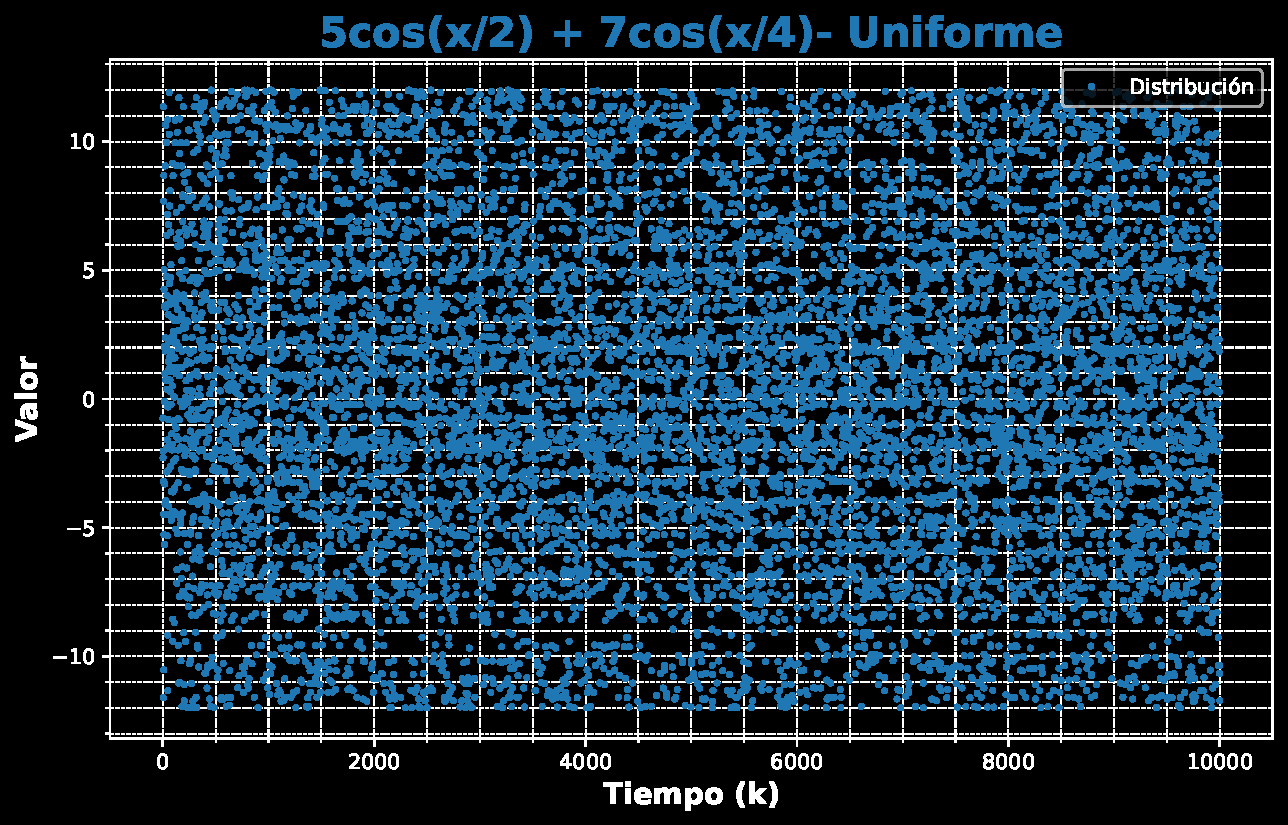
\includegraphics[width=\textwidth]{per_uniforme1} % Asegúrate de cambiar la ruta a la ubicación de tu imagen
				\caption{Gráfica de la serie de tiempo para la función \( 5\cdot \cos\left(\frac{x}{2}\right) + 7\cdot \cos\left(\frac{x^2}{4}\right) \).}
			\end{figure}
		\end{column}
		
		% Columna de la derecha
		\begin{column}{0.5\textwidth} % Ajusta la proporción según necesites
			\begin{figure}
				\centering
				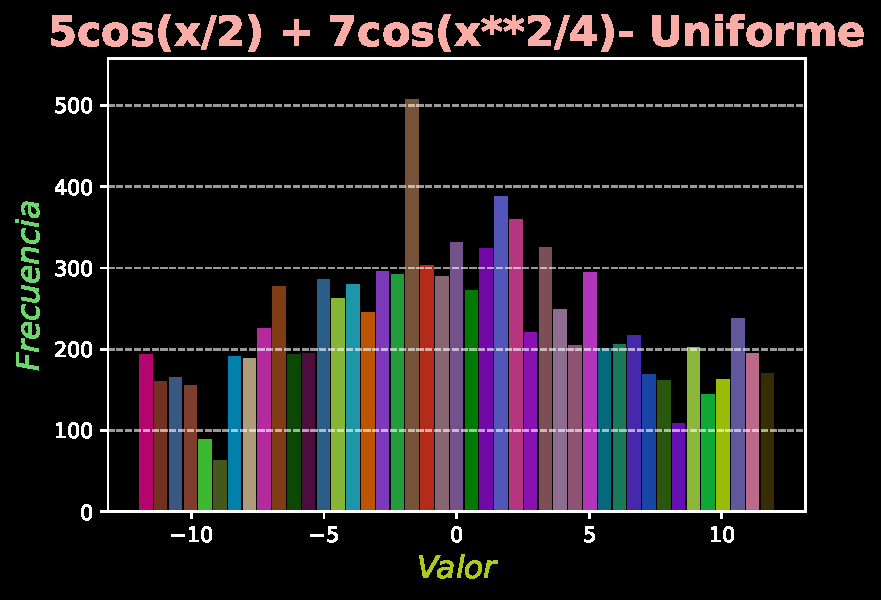
\includegraphics[width=\textwidth]{per_uniforme2} % Asegúrate de cambiar la ruta a la ubicación de tu imagen
				\caption{Distribución de los datos.}
			\end{figure}
		\end{column}
	\end{columns}
\end{frame}


%------------------------------------------------



\section{Caminante Aleatorio}


\begin{frame}
	\frametitle{Caminante Aleatorio}
	\begin{figure}
		\centering
		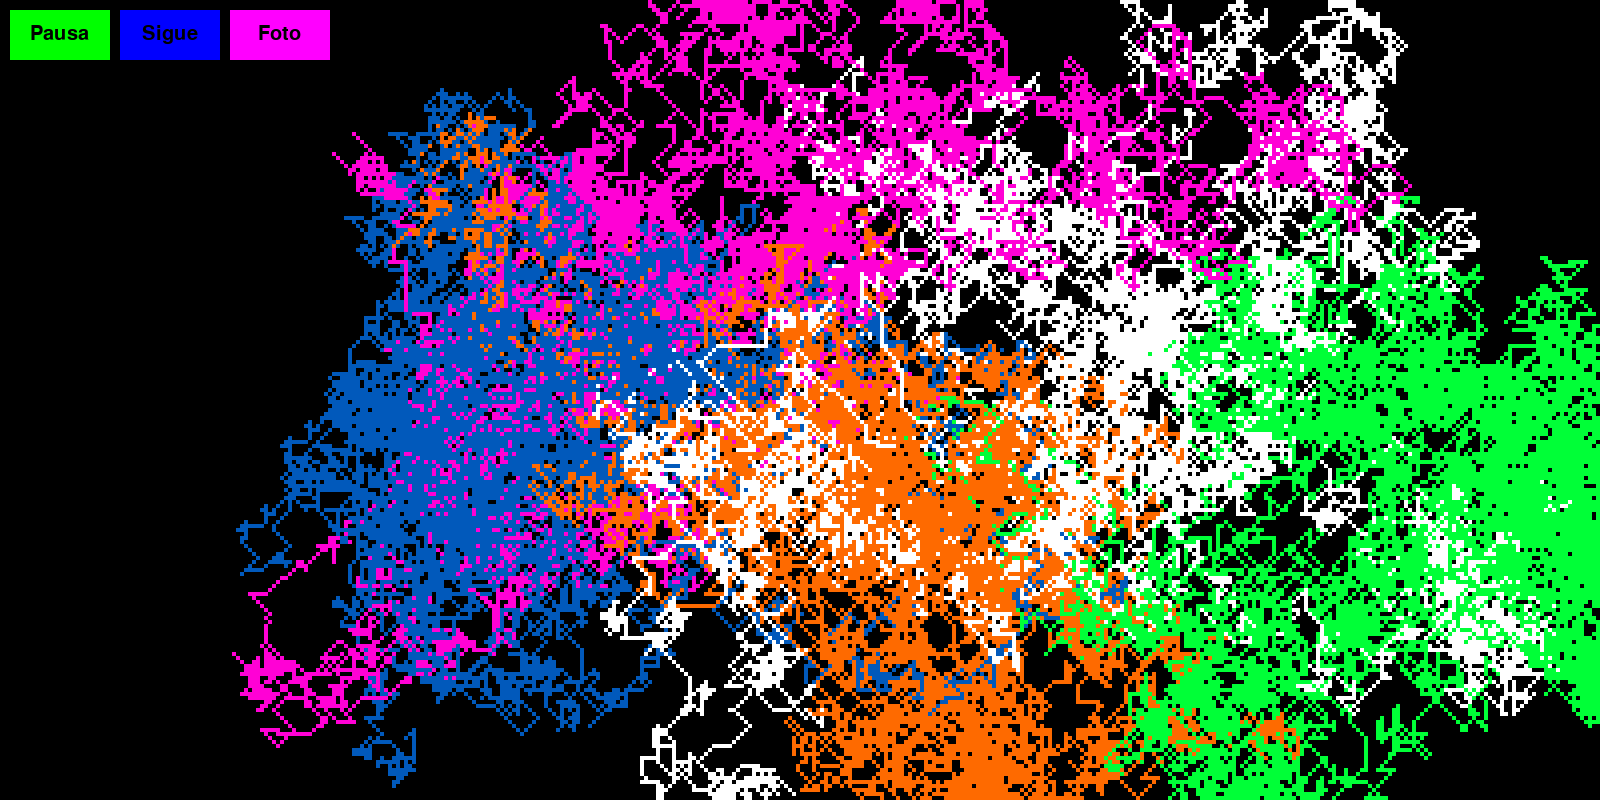
\includegraphics[width=\textwidth]{walkerUniforme} % Asegúrate de cambiar la ruta a la ubicación de tu imagen
		\caption{Caminante Aleatorio con distribución uniforme}
	\end{figure}
	
	
\end{frame}

\begin{frame}
	\frametitle{Caminante Aleatorio}
	Utilizando datos generados según distribuciones uniforme (\texttt{randomsUniforme.txt}), normal (\texttt{randomsNormal.txt}), y gamma (\texttt{randomsGamma.txt}), se propone crear una animación de caminante aleatorio. El objetivo es examinar cómo las diferentes distribuciones de probabilidad influyen en el comportamiento del caminante y en las series de tiempo derivadas. Se analizarán las siguientes métricas:
	
	\vspace{5mm}
	\begin{itemize}
		\item Dirección y distancia de cada paso.
		\item Incidencias de choques con obstáculos.
		\item Evolución de la posición (x,y) en el plano.
	\end{itemize}
	
\end{frame}


\begin{frame}
	\frametitle{Caminante Aleatorio - Datos Uniformes}
	\begin{figure}
		\centering
		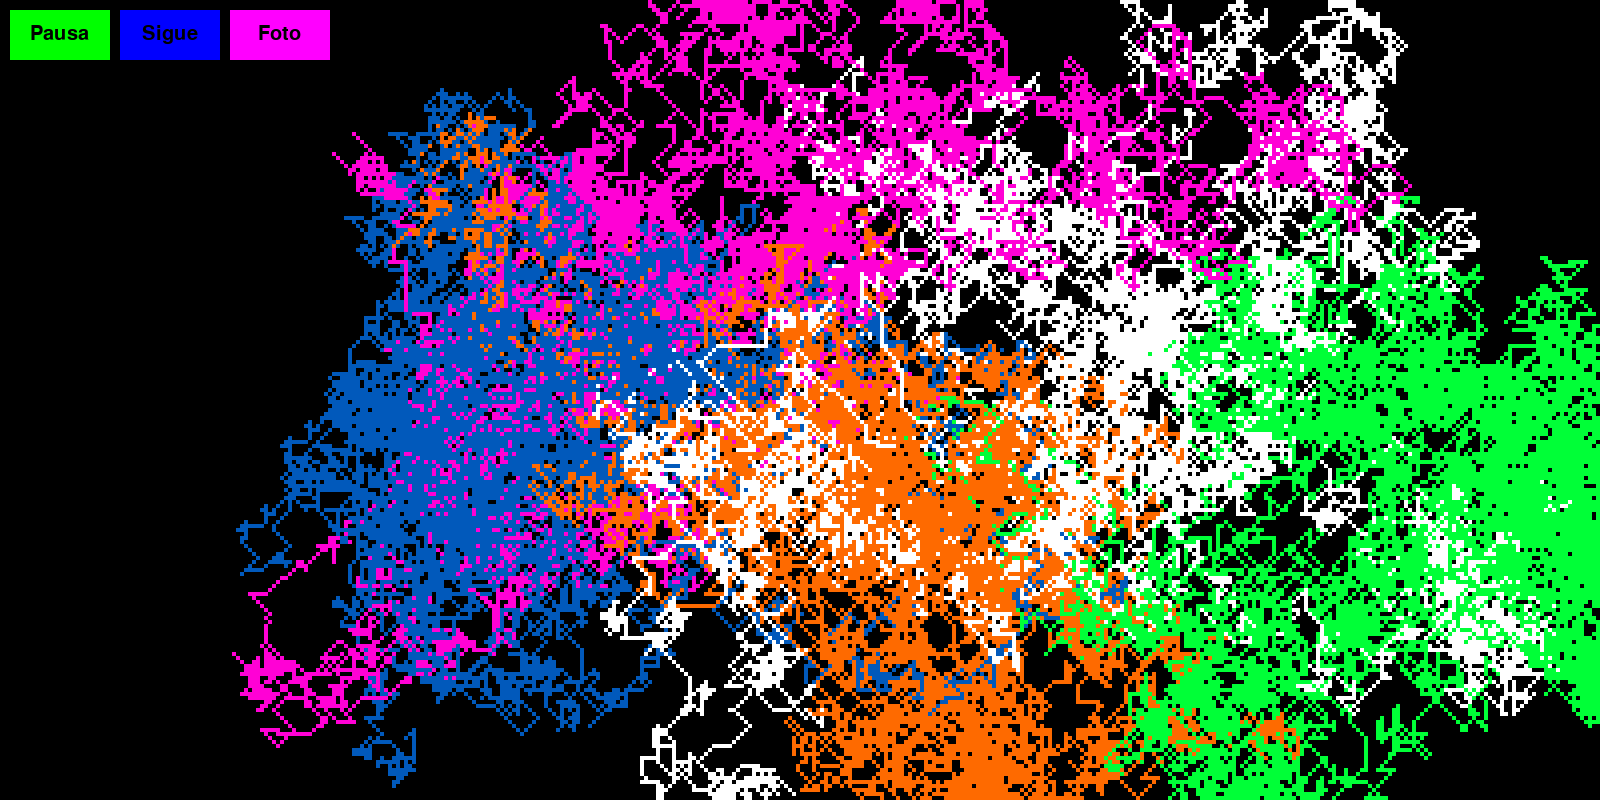
\includegraphics[width=\textwidth]{walkerUniforme} % Asegúrate de cambiar la ruta a la ubicación de tu imagen
		\caption{Caminante Aleatorio con distribución uniforme}
	\end{figure}
\end{frame}

\begin{frame}
	\frametitle{Gamma - Uniforme}
	
	\begin{columns}
		
		% Columna de la izquierda
		\begin{column}{0.5\textwidth} % Ajusta la proporción según necesites
			\begin{figure}
				\centering
				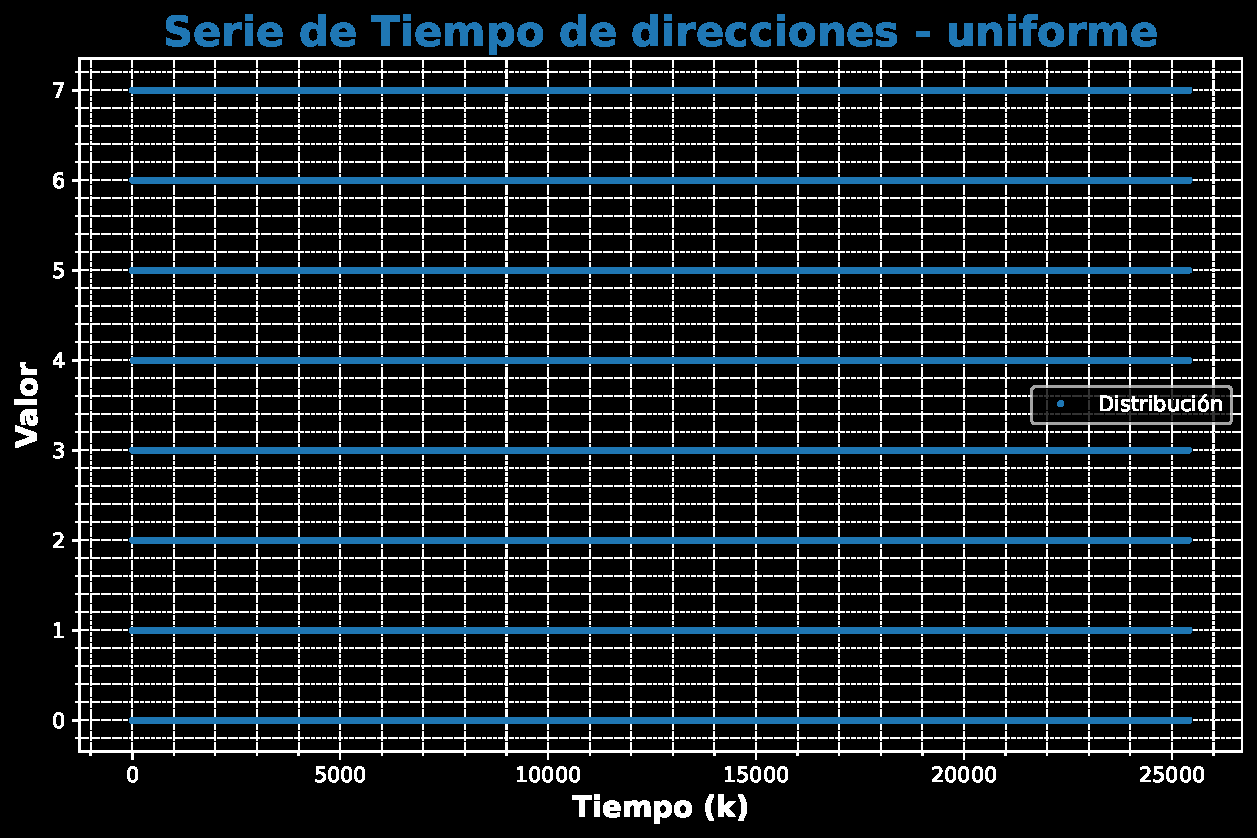
\includegraphics[width=\textwidth]{graf_direcciones_uniforme} % Asegúrate de cambiar la ruta a la ubicación de tu imagen
				\caption{Gráfica de la serie de tiempo para las direcciones.}
			\end{figure}
		\end{column}
		
		% Columna de la derecha
		\begin{column}{0.5\textwidth} % Ajusta la proporción según necesites
			\begin{figure}
				\centering
				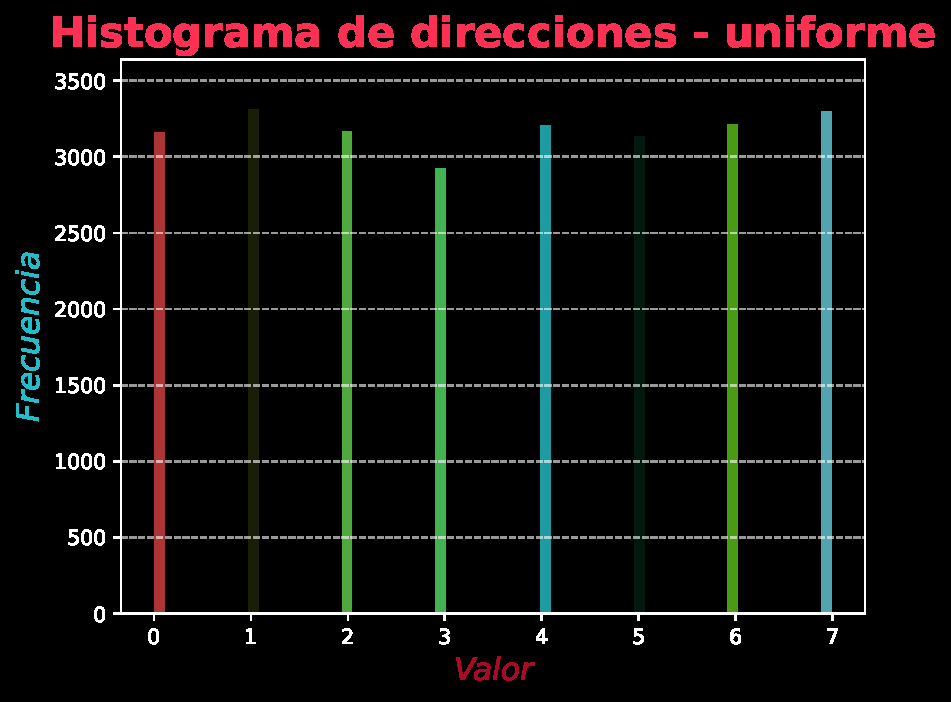
\includegraphics[width=\textwidth]{hist_direcciones_uniforme} % Asegúrate de cambiar la ruta a la ubicación de tu imagen
				\caption{Histograma de los datos de direcciones.}
			\end{figure}
		\end{column}
	\end{columns}
\end{frame}


\begin{frame}
	\frametitle{Caminante Aleatorio - Datos Normal}
	\begin{figure}
		\centering
		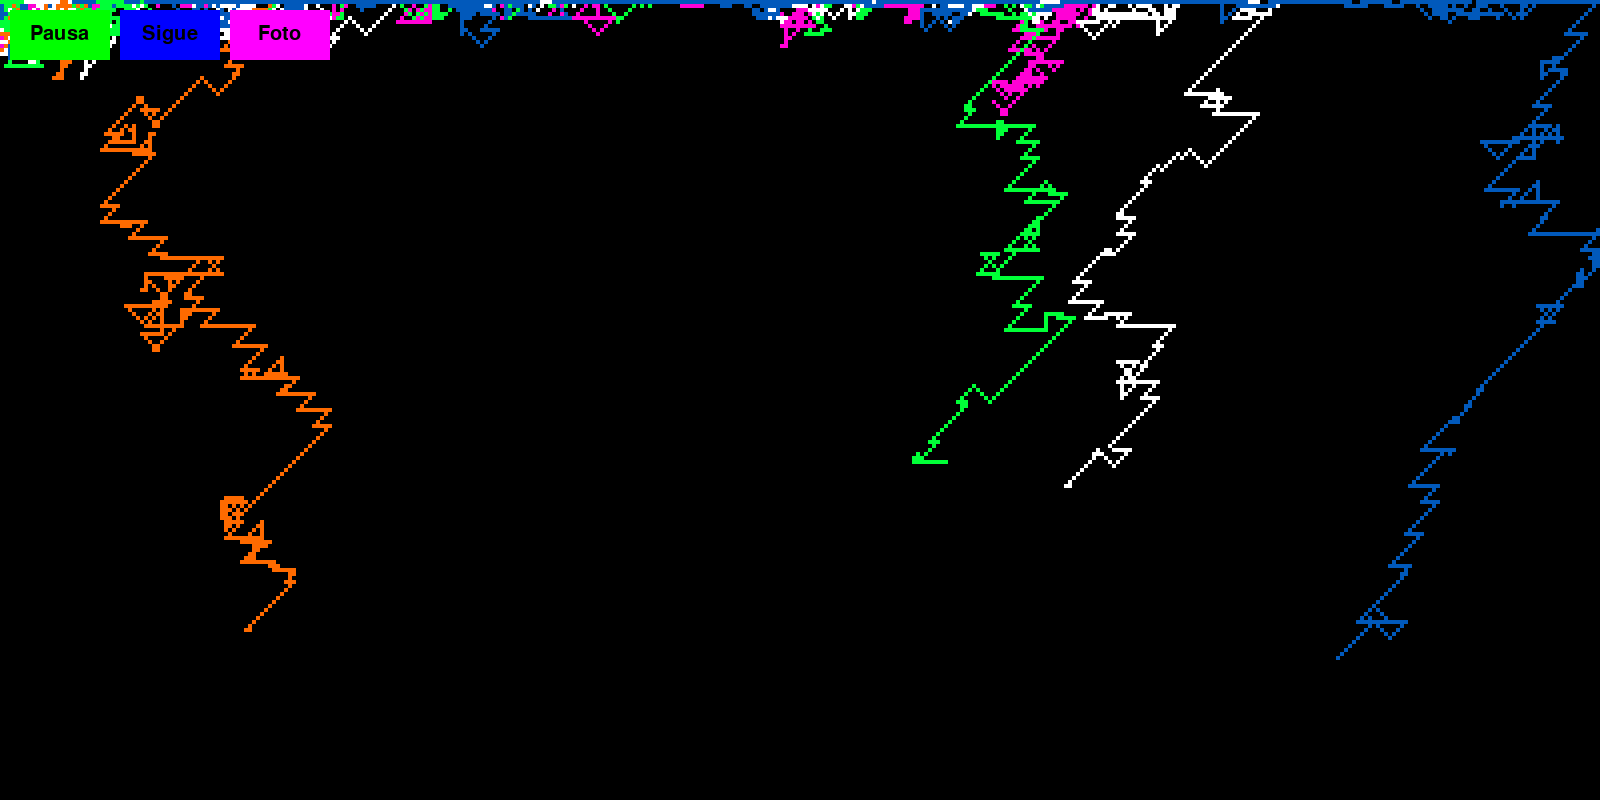
\includegraphics[width=\textwidth]{walkerNormal} % Asegúrate de cambiar la ruta a la ubicación de tu imagen
		\caption{Caminante Aleatorio con distribución normal}
	\end{figure}
\end{frame}

\begin{frame}
	\frametitle{Gamma - Normal}
	
	\begin{columns}
		
		% Columna de la izquierda
		\begin{column}{0.5\textwidth} % Ajusta la proporción según necesites
			\begin{figure}
				\centering
				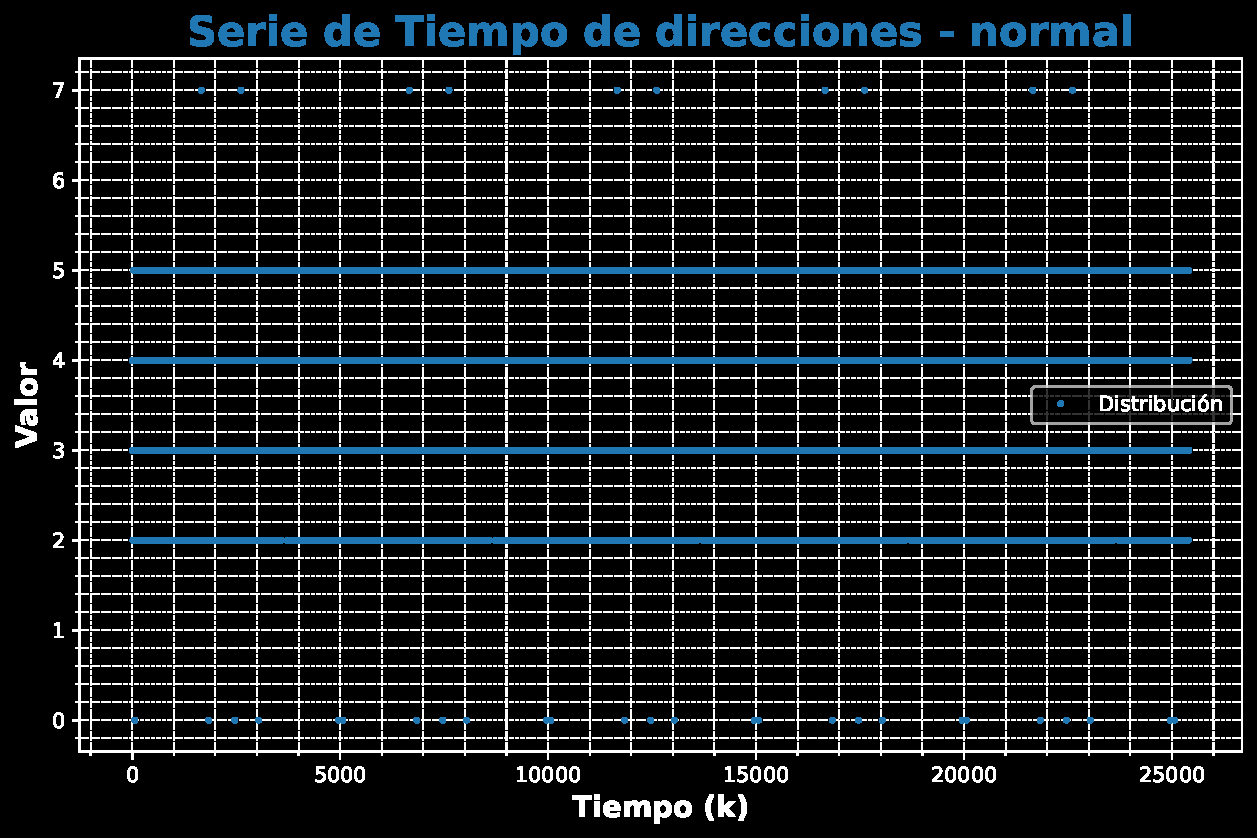
\includegraphics[width=\textwidth]{graf_direcciones_normal} % Asegúrate de cambiar la ruta a la ubicación de tu imagen
				\caption{Gráfica de la serie de tiempo para las direcciones.}
			\end{figure}
		\end{column}
		
		% Columna de la derecha
		\begin{column}{0.5\textwidth} % Ajusta la proporción según necesites
			\begin{figure}
				\centering
				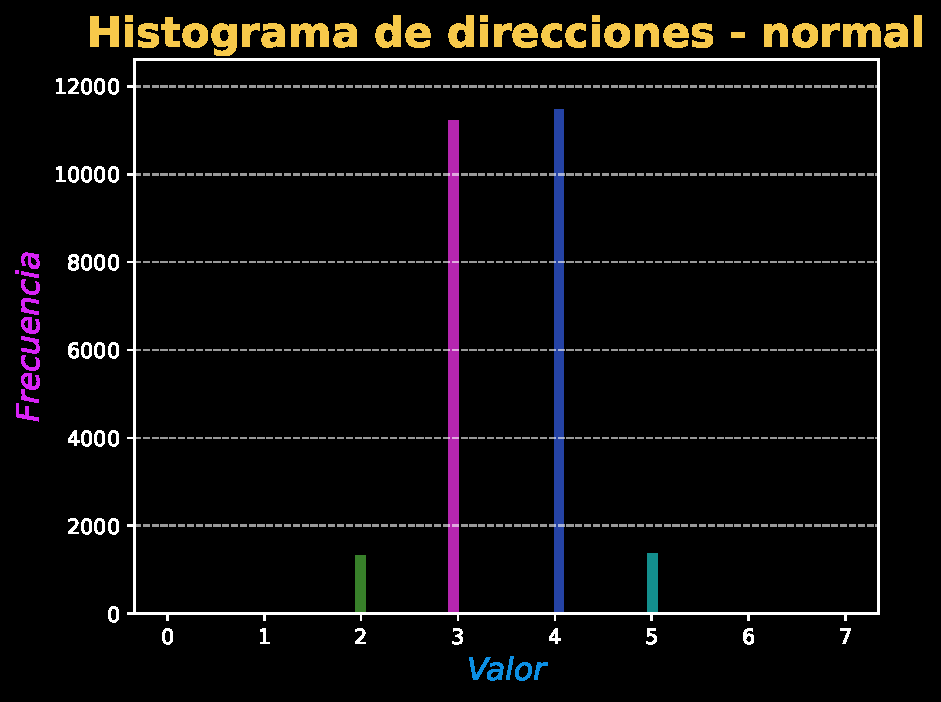
\includegraphics[width=\textwidth]{hist_direcciones_normal} % Asegúrate de cambiar la ruta a la ubicación de tu imagen
				\caption{Histograma de los datos de direcciones.}
			\end{figure}
		\end{column}
	\end{columns}
\end{frame}


\begin{frame}
	\frametitle{Caminante Aleatorio - Datos Gamma}
	\begin{figure}
		\centering
		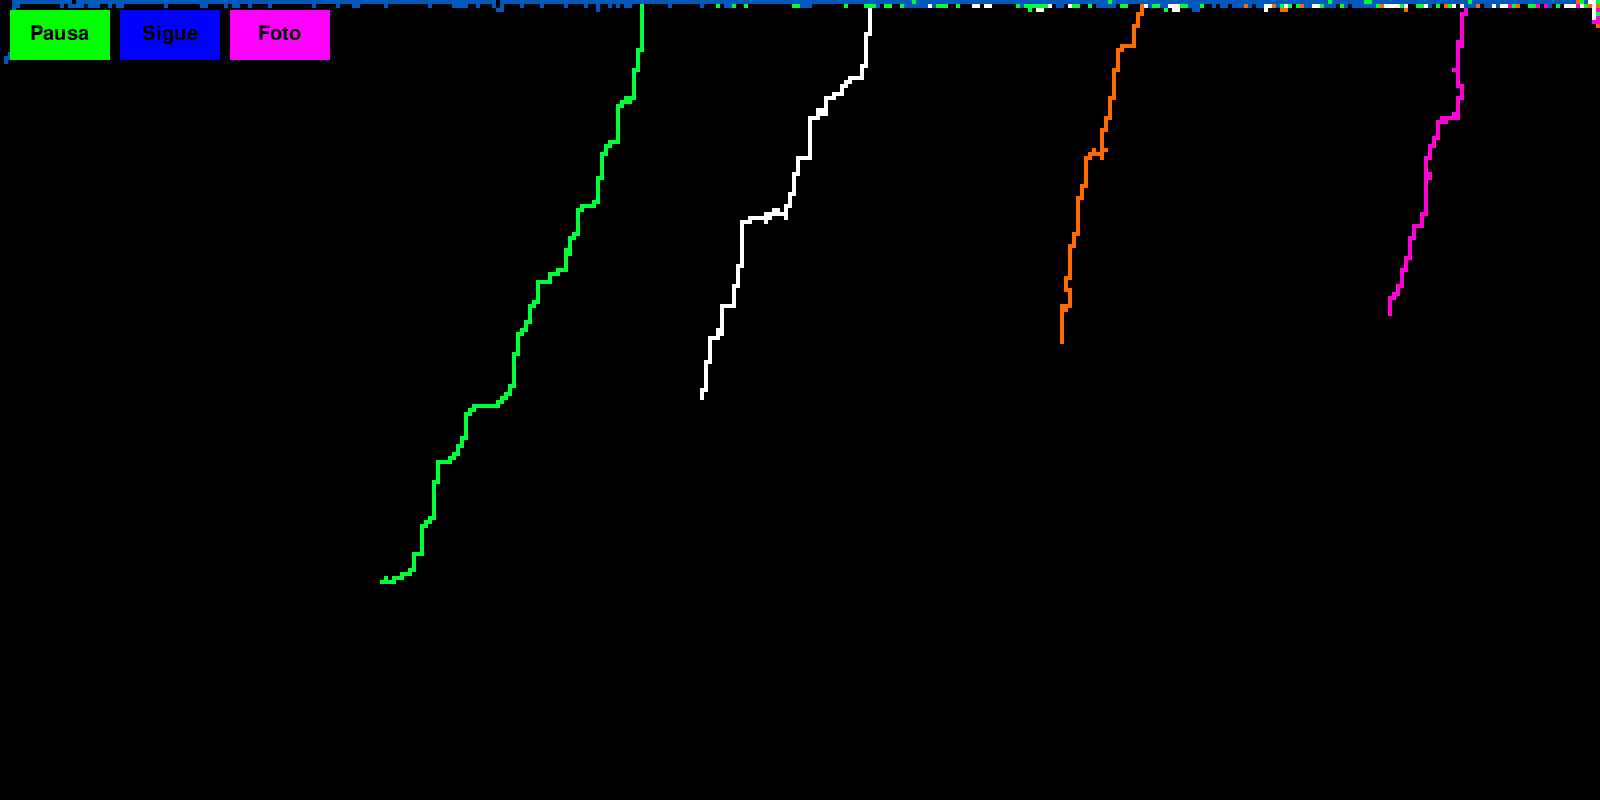
\includegraphics[width=\textwidth]{walkerGamma} % Asegúrate de cambiar la ruta a la ubicación de tu imagen
		\caption{Caminante Aleatorio con distribución gamma}
	\end{figure}
\end{frame}



\begin{frame}
	\frametitle{Gamma - Direcciones}
	
	\begin{columns}
		
		% Columna de la izquierda
		\begin{column}{0.5\textwidth} % Ajusta la proporción según necesites
			\begin{figure}
				\centering
				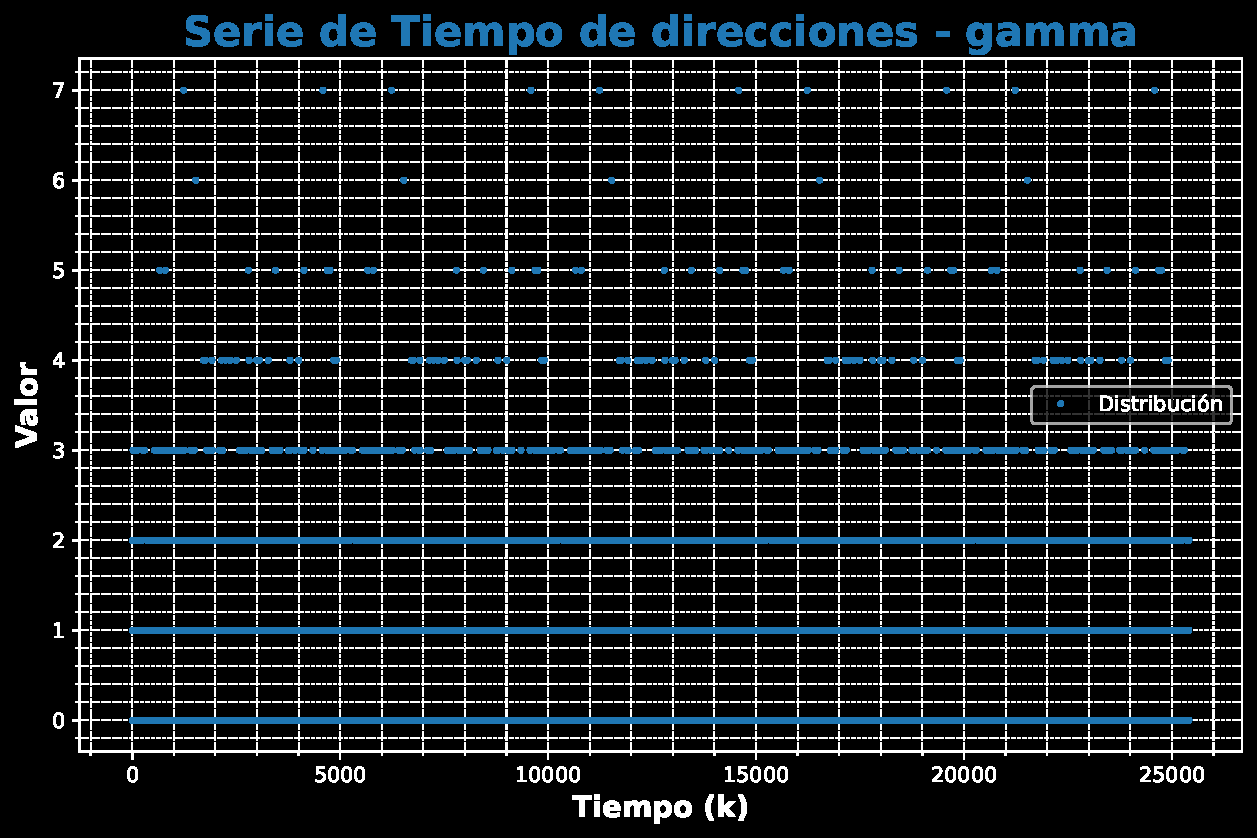
\includegraphics[width=\textwidth]{graf_direcciones_gamma} % Asegúrate de cambiar la ruta a la ubicación de tu imagen
				\caption{Gráfica de la serie de tiempo para las direcciones.}
			\end{figure}
		\end{column}
		
		% Columna de la derecha
		\begin{column}{0.5\textwidth} % Ajusta la proporción según necesites
			\begin{figure}
				\centering
				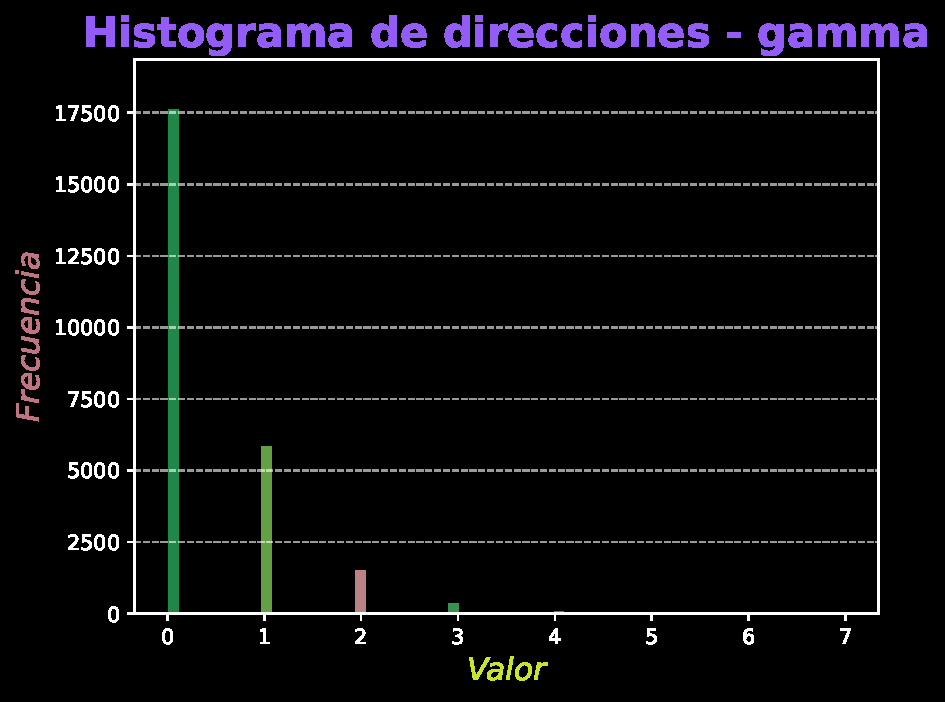
\includegraphics[width=\textwidth]{hist_direcciones_gamma} % Asegúrate de cambiar la ruta a la ubicación de tu imagen
				\caption{Histograma de los datos de direcciones.}
			\end{figure}
		\end{column}
	\end{columns}
\end{frame}


%----------------------------------------------------------------------------------------
%	CLOSING SLIDE
%----------------------------------------------------------------------------------------

\begin{frame}[plain] % The optional argument 'plain' hides the headline and footline
	\begin{center}
		\vspace{15mm}
		{\Huge ¡Gracias!}
	\end{center}
\end{frame}

%----------------------------------------------------------------------------------------

\end{document} 